%\nosectionpage
\section{The Things Network (Präsentationsschicht)}
%\withsectionpage

\begin{frame}{\href{https://www.thethingsnetwork.org/}{The Things Network (\alert{TTN})}}
  \begin{center}
    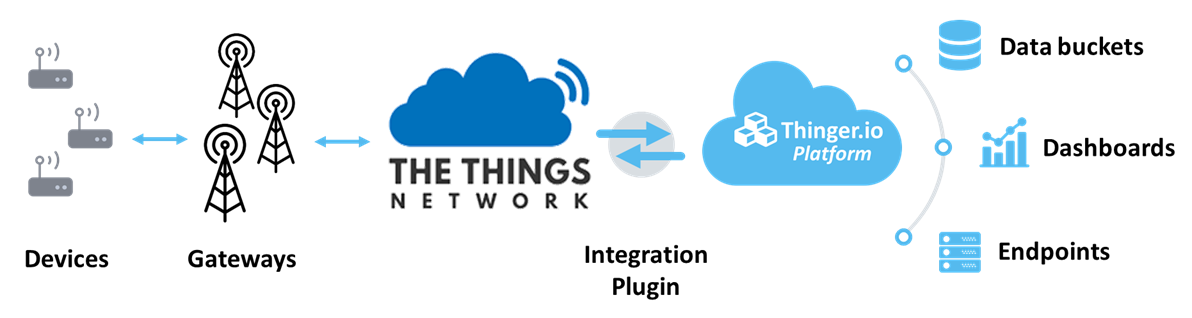
\includegraphics[width=0.7\textwidth]{material/the-things-network.png}
  \end{center}
  \begin{itemize}
\item Globale, Community-getriebene Open-Source-Initiative.
\item Stellt eine dezentrale Infrastruktur für das Internet der Dinge bereit.
\item Verwendet das LoRaWAN-Protokoll.
\item Bietet unterschiedliche Integrationstechniken über Plugins
    \begin{itemize}
\item MQTT
\item Amazon AWS IoT
\item Microsoft Azure IoT
\item Webhooks
\item LoRa Cloud
\item Storage Integration
    \end{itemize}
  \end{itemize}
\end{frame}
